\documentclass[11pt,compress,t,notes=noshow, xcolor=table]{beamer}
\usepackage[]{graphicx}
\usepackage[]{color}
% maxwidth is the original width if it is less than linewidth
% otherwise use linewidth (to make sure the graphics do not exceed the margin)
\makeatletter
\def\maxwidth{ %
  \ifdim\Gin@nat@width>\linewidth
    \linewidth
  \else
    \Gin@nat@width
  \fi
}
\makeatother

% ---------------------------------%
% latex-math dependencies, do not remove:
% - \usepackage{mathtools}
% - \usepackage{bm}
% - \usepackage{siunitx}
% - \usepackage{dsfont}
% - \usepackage{xspace}
% ---------------------------------%

%--------------------------------------------------------%
%       Language, encoding, typography
%--------------------------------------------------------%

\usepackage[english]{babel}
\usepackage[utf8]{inputenc} % Enables inputting UTF-8 symbols
% Standard AMS suite
\usepackage{amsmath,amsfonts,amssymb}

% Font four double-stroke / blackboard letters for sets of numbers (N, R, ...)
% Distribution name is "doublestroke"
% According to https://mirror.physik.tu-berlin.de/pub/CTAN/fonts/doublestroke/dsdoc.pdf
% the "bbm" package does a similar thing and may be superfluous.
% Required for latex-math
\usepackage{dsfont}

% bbm – "Blackboard-style" cm fonts (https://www.ctan.org/pkg/bbm)
% Used to be in common.tex, loaded directly after this file
% Maybe superfluous given dsfont is loaded
% TODO: Check if really unused?
% \usepackage{bbm}

% bm – Access bold symbols in maths mode - https://ctan.org/pkg/bm
% Required for latex-math
% https://tex.stackexchange.com/questions/3238/bm-package-versus-boldsymbol
\usepackage{bm}

% pifont – Access to PostScript standard Symbol and Dingbats fonts
% Used for \newcommand{\xmark}{\ding{55}, which is never used
% aside from lecture_advml/attic/xx-automl/slides.Rnw
% \usepackage{pifont}

% Quotes (inline and display), provdes \enquote
% https://ctan.org/pkg/csquotes
\usepackage{csquotes}

% Adds arg to enumerate env, technically superseded by enumitem according
% to https://ctan.org/pkg/enumerate
% Replace with https://ctan.org/pkg/enumitem ?
\usepackage{enumerate}

% Line spacing - provides \singlespacing \doublespacing \onehalfspacing
% https://ctan.org/pkg/setspace
% TODO: Check if really unused?
%\usepackage{setspace}

% mathtools – Mathematical tools to use with amsmath
% https://ctan.org/pkg/mathtools?lang=en
% latex-math dependency according to latex-math repo
\usepackage{mathtools}

%--------------------------------------------------------%
%       Displaying code and algorithms
%--------------------------------------------------------%
\usepackage{verbatim}
\usepackage{algorithm}
\usepackage{algpseudocode}

%--------------------------------------------------------%
%       Tables
%--------------------------------------------------------%

% multi-row table cells: https://www.namsu.de/Extra/pakete/Multirow.html
\usepackage{multirow}

% long/multi-page tables: https://texdoc.org/serve/longtable.pdf/0
% TODO: Check if really unused?

\usepackage{longtable}

% pretty table env: https://ctan.org/pkg/booktabs?lang=en
% TODO: Check if really unused?
\usepackage{booktabs}

%--------------------------------------------------------%
%       Figures: Creating, placing, verbing
%--------------------------------------------------------%

% wrapfig - Wrapping text around figures https://de.overleaf.com/learn/latex/Wrapping_text_around_figures
\usepackage{wrapfig}

% Sub figures in figures and tables
% https://ctan.org/pkg/subfig -- supersedes subfigure package
% TODO: Check if really unused?
\usepackage{subfig}

% Actually it's pronounced PGF https://en.wikibooks.org/wiki/LaTeX/PGF/TikZ
\usepackage{tikz}

\usetikzlibrary{shapes,arrows,automata,positioning,calc,chains,trees, shadows}
\tikzset{
  %Define standard arrow tip
  >=stealth',
  %Define style for boxes
  punkt/.style={
    rectangle,
    rounded corners,
    draw=black, very thick,
    text width=6.5em,
    minimum height=2em,
    text centered},
  % Define arrow style
  pil/.style={
    ->,
    thick,
    shorten <=2pt,
    shorten >=2pt,}
}


% Unsorted
% textpos – Place boxes at arbitrary positions on the LATEX page
% https://ctan.org/pkg/textpos?lang=en
% Provides \begin{textblock}
 % TODO: Check if really unused?
\usepackage[absolute,overlay]{textpos}

% psfrag – Replace strings in encapsulated PostScript figures
% https://www.overleaf.com/latex/examples/psfrag-example/tggxhgzwrzhn
% https://ftp.mpi-inf.mpg.de/pub/tex/mirror/ftp.dante.de/pub/tex/macros/latex/contrib/psfrag/pfgguide.pdf
% Can't tell if this is needed
% TODO: Check if really unused?
\usepackage{psfrag}

% Maybe not great to use this https://tex.stackexchange.com/a/197/19093
% Use align instead -- TODO: Global search & replace to check
\usepackage{eqnarray}

\usepackage{colortbl}

% arydshln – Draw dash-lines in array/tabular
% https://www.ctan.org/pkg/arydshln
% !! "arydshln has to be loaded after array, longtable, colortab and/or colortbl"
% Provides \hdashline and \cdashline
% TODO: Check if really unused?
% \usepackage{arydshln}

% tabularx – Tabulars with adjustable-width columns
% https://ctan.org/pkg/tabularx
% Provides \begin{tabularx}
% TODO: Check if really unused?
% \usepackage{tabularx}

% placeins – Control float placement
% https://ctan.org/pkg/placeins
% Defines a \FloatBarrier command
% TODO: Check if really unused?
% \usepackage{placeins}


% framed – Framed or shaded regions that can break across pages
% https://ctan.org/pkg/framed
% Provides \begin{framed} which uses \colorbox{shadecolor} relying on \definecolor{shadecolor}.
% TODO: Check if really unused?
% \usepackage{framed}

% Used often in conjunction with \definecolor{shadecolor}{rgb}{0.969, 0.969, 0.969}
% Might be able to be removed or at least redefined to only have shadecolor (if needed)
\definecolor{fgcolor}{rgb}{0.345, 0.345, 0.345}
\definecolor{shadecolor}{rgb}{0.969, 0.969, 0.969}
\newenvironment{knitrout}{}{} % an empty environment to be redefined in TeX


% Defines macros and environments
\usepackage{../../style/lmu-lecture}

\let\code=\texttt % Used regularly
\let\proglang=\textsf % Unused?

% Not sure what/why this does
\setkeys{Gin}{width=0.9\textwidth}

\setbeamertemplate{frametitle}{\expandafter\uppercase\expandafter\insertframetitle}

% Can't find a reason why common.tex is not just part of this file?
% Rarely used fontstyle for R packages, used only in 
% - forests/slides-forests-benchmark.tex
% - exercises/single-exercises/methods_l_1.Rnw
% - slides/cart/attic/slides_extra_trees.Rnw
\newcommand{\pkg}[1]{{\fontseries{b}\selectfont #1}}

% Spacing helpers, used often (mostly in exercises for \dlz)
\newcommand{\lz}{\vspace{0.5cm}} % vertical space (used often in slides)
\newcommand{\dlz}{\vspace{1cm}}  % double vertical space (used often in exercises, never in slides)

%--------------------%
%  New environments  %
%--------------------%

 % Frame with breaks and verbatim // this is used very often
\newenvironment{vbframe}
{
\begin{frame}[containsverbatim,allowframebreaks]
}
{
\end{frame}
}

% Frame with verbatim without breaks (to avoid numbering one slided frames)
% This is not used anywhere but I can see it being useful
\newenvironment{vframe}
{
\begin{frame}[containsverbatim]
}
{
\end{frame}
}

% Itemize block
\newenvironment{blocki}[1]
{
\begin{block}{#1}\begin{itemize}
}
{
\end{itemize}\end{block}
}

% textcolor that works in mathmode
% https://tex.stackexchange.com/a/261480
% Used e.g. in forests/slides-forests-bagging.tex
% [...] \textcolor{blue}{\tfrac{1}{M}\sum^M_{m} [...]
% \makeatletter
% \renewcommand*{\@textcolor}[3]{%
%   \protect\leavevmode
%   \begingroup
%     \color#1{#2}#3%
%   \endgroup
% }
% \makeatother


%-------------------------------------------------------------------------------------------------------%
%  Unused stuff that needs to go but is kept here currently juuuust in case it was important after all  %
%-------------------------------------------------------------------------------------------------------%

% \newcommand{\hlnum}[1]{\textcolor[rgb]{0.686,0.059,0.569}{#1}}%
% \newcommand{\hlstr}[1]{\textcolor[rgb]{0.192,0.494,0.8}{#1}}%
% \newcommand{\hlcom}[1]{\textcolor[rgb]{0.678,0.584,0.686}{\textit{#1}}}%
% \newcommand{\hlopt}[1]{\textcolor[rgb]{0,0,0}{#1}}%
% \newcommand{\hlstd}[1]{\textcolor[rgb]{0.345,0.345,0.345}{#1}}%
% \newcommand{\hlkwa}[1]{\textcolor[rgb]{0.161,0.373,0.58}{\textbf{#1}}}%
% \newcommand{\hlkwb}[1]{\textcolor[rgb]{0.69,0.353,0.396}{#1}}%
% \newcommand{\hlkwc}[1]{\textcolor[rgb]{0.333,0.667,0.333}{#1}}%
% \newcommand{\hlkwd}[1]{\textcolor[rgb]{0.737,0.353,0.396}{\textbf{#1}}}%
% \let\hlipl\hlkwb

% \makeatletter
% \newenvironment{kframe}{%
%  \def\at@end@of@kframe{}%
%  \ifinner\ifhmode%
%   \def\at@end@of@kframe{\end{minipage}}%
%   \begin{minipage}{\columnwidth}%
%  \fi\fi%
%  \def\FrameCommand##1{\hskip\@totalleftmargin \hskip-\fboxsep
%  \colorbox{shadecolor}{##1}\hskip-\fboxsep
%      % There is no \\@totalrightmargin, so:
%      \hskip-\linewidth \hskip-\@totalleftmargin \hskip\columnwidth}%
%  \MakeFramed {\advance\hsize-\width
%    \@totalleftmargin\z@ \linewidth\hsize
%    \@setminipage}}%
%  {\par\unskip\endMakeFramed%
%  \at@end@of@kframe}
% \makeatother

% \definecolor{shadecolor}{rgb}{.97, .97, .97}
% \definecolor{messagecolor}{rgb}{0, 0, 0}
% \definecolor{warningcolor}{rgb}{1, 0, 1}
% \definecolor{errorcolor}{rgb}{1, 0, 0}
% \newenvironment{knitrout}{}{} % an empty environment to be redefined in TeX

% \usepackage{alltt}
% \newcommand{\SweaveOpts}[1]{}  % do not interfere with LaTeX
% \newcommand{\SweaveInput}[1]{} % because they are not real TeX commands
% \newcommand{\Sexpr}[1]{}       % will only be parsed by R
% \newcommand{\xmark}{\ding{55}}%

% dependencies: amsmath, amssymb, dsfont
% math spaces
\ifdefined\N
\renewcommand{\N}{\mathds{N}} % N, naturals
\else \newcommand{\N}{\mathds{N}} \fi
\newcommand{\Z}{\mathds{Z}} % Z, integers
\newcommand{\Q}{\mathds{Q}} % Q, rationals
\newcommand{\R}{\mathds{R}} % R, reals
\ifdefined\C
\renewcommand{\C}{\mathds{C}} % C, complex
\else \newcommand{\C}{\mathds{C}} \fi
\newcommand{\continuous}{\mathcal{C}} % C, space of continuous functions
\newcommand{\M}{\mathcal{M}} % machine numbers
\newcommand{\epsm}{\epsilon_m} % maximum error

% counting / finite sets
\newcommand{\setzo}{\{0, 1\}} % set 0, 1
\newcommand{\setmp}{\{-1, +1\}} % set -1, 1
\newcommand{\unitint}{[0, 1]} % unit interval

% basic math stuff
\newcommand{\xt}{\tilde x} % x tilde
\DeclareMathOperator*{\argmax}{arg\,max} % argmax
\DeclareMathOperator*{\argmin}{arg\,min} % argmin
\newcommand{\argminlim}{\mathop{\mathrm{arg\,min}}\limits} % argmax with limits
\newcommand{\argmaxlim}{\mathop{\mathrm{arg\,max}}\limits} % argmin with limits
\newcommand{\sign}{\operatorname{sign}} % sign, signum
\newcommand{\I}{\mathbb{I}} % I, indicator
\newcommand{\order}{\mathcal{O}} % O, order
\newcommand{\bigO}{\mathcal{O}} % Big-O Landau
\newcommand{\littleo}{{o}} % Little-o Landau
\newcommand{\pd}[2]{\frac{\partial{#1}}{\partial #2}} % partial derivative
\newcommand{\floorlr}[1]{\left\lfloor #1 \right\rfloor} % floor
\newcommand{\ceillr}[1]{\left\lceil #1 \right\rceil} % ceiling
\newcommand{\indep}{\perp \!\!\! \perp} % independence symbol

% sums and products
\newcommand{\sumin}{\sum\limits_{i=1}^n} % summation from i=1 to n
\newcommand{\sumim}{\sum\limits_{i=1}^m} % summation from i=1 to m
\newcommand{\sumjn}{\sum\limits_{j=1}^n} % summation from j=1 to p
\newcommand{\sumjp}{\sum\limits_{j=1}^p} % summation from j=1 to p
\newcommand{\sumik}{\sum\limits_{i=1}^k} % summation from i=1 to k
\newcommand{\sumkg}{\sum\limits_{k=1}^g} % summation from k=1 to g
\newcommand{\sumjg}{\sum\limits_{j=1}^g} % summation from j=1 to g
\newcommand{\meanin}{\frac{1}{n} \sum\limits_{i=1}^n} % mean from i=1 to n
\newcommand{\meanim}{\frac{1}{m} \sum\limits_{i=1}^m} % mean from i=1 to n
\newcommand{\meankg}{\frac{1}{g} \sum\limits_{k=1}^g} % mean from k=1 to g
\newcommand{\prodin}{\prod\limits_{i=1}^n} % product from i=1 to n
\newcommand{\prodkg}{\prod\limits_{k=1}^g} % product from k=1 to g
\newcommand{\prodjp}{\prod\limits_{j=1}^p} % product from j=1 to p

% linear algebra
\newcommand{\one}{\bm{1}} % 1, unitvector
\newcommand{\zero}{\mathbf{0}} % 0-vector
\newcommand{\id}{\bm{I}} % I, identity
\newcommand{\diag}{\operatorname{diag}} % diag, diagonal
\newcommand{\trace}{\operatorname{tr}} % tr, trace
\newcommand{\spn}{\operatorname{span}} % span
\newcommand{\scp}[2]{\left\langle #1, #2 \right\rangle} % <.,.>, scalarproduct
\newcommand{\mat}[1]{\begin{pmatrix} #1 \end{pmatrix}} % short pmatrix command
\newcommand{\Amat}{\mathbf{A}} % matrix A
\newcommand{\Deltab}{\mathbf{\Delta}} % error term for vectors

% basic probability + stats
\renewcommand{\P}{\mathds{P}} % P, probability
\newcommand{\E}{\mathds{E}} % E, expectation
\newcommand{\var}{\mathsf{Var}} % Var, variance
\newcommand{\cov}{\mathsf{Cov}} % Cov, covariance
\newcommand{\corr}{\mathsf{Corr}} % Corr, correlation
\newcommand{\normal}{\mathcal{N}} % N of the normal distribution
\newcommand{\iid}{\overset{i.i.d}{\sim}} % dist with i.i.d superscript
\newcommand{\distas}[1]{\overset{#1}{\sim}} % ... is distributed as ...

% machine learning
\newcommand{\Xspace}{\mathcal{X}} % X, input space
\newcommand{\Yspace}{\mathcal{Y}} % Y, output space
\newcommand{\Zspace}{\mathcal{Z}} % Space of sampled datapoints ! Also defined identically in ml-online.tex !
\newcommand{\nset}{\{1, \ldots, n\}} % set from 1 to n
\newcommand{\pset}{\{1, \ldots, p\}} % set from 1 to p
\newcommand{\gset}{\{1, \ldots, g\}} % set from 1 to g
\newcommand{\Pxy}{\mathbb{P}_{xy}} % P_xy
\newcommand{\Exy}{\mathbb{E}_{xy}} % E_xy: Expectation over random variables xy
\newcommand{\xv}{\mathbf{x}} % vector x (bold)
\newcommand{\xtil}{\tilde{\mathbf{x}}} % vector x-tilde (bold)
\newcommand{\yv}{\mathbf{y}} % vector y (bold)
\newcommand{\xy}{(\xv, y)} % observation (x, y)
\newcommand{\xvec}{\left(x_1, \ldots, x_p\right)^\top} % (x1, ..., xp)
\newcommand{\Xmat}{\mathbf{X}} % Design matrix
\newcommand{\allDatasets}{\mathds{D}} % The set of all datasets
\newcommand{\allDatasetsn}{\mathds{D}_n}  % The set of all datasets of size n
\newcommand{\D}{\mathcal{D}} % D, data
\newcommand{\Dn}{\D_n} % D_n, data of size n
\newcommand{\Dtrain}{\mathcal{D}_{\text{train}}} % D_train, training set
\newcommand{\Dtest}{\mathcal{D}_{\text{test}}} % D_test, test set
\newcommand{\xyi}[1][i]{\left(\xv^{(#1)}, y^{(#1)}\right)} % (x^i, y^i), i-th observation
\newcommand{\Dset}{\left( \xyi[1], \ldots, \xyi[n]\right)} % {(x1,y1)), ..., (xn,yn)}, data
\newcommand{\defAllDatasetsn}{(\Xspace \times \Yspace)^n} % Def. of the set of all datasets of size n
\newcommand{\defAllDatasets}{\bigcup_{n \in \N}(\Xspace \times \Yspace)^n} % Def. of the set of all datasets
\newcommand{\xdat}{\left\{ \xv^{(1)}, \ldots, \xv^{(n)}\right\}} % {x1, ..., xn}, input data
\newcommand{\ydat}{\left\{ \yv^{(1)}, \ldots, \yv^{(n)}\right\}} % {y1, ..., yn}, input data
\newcommand{\yvec}{\left(y^{(1)}, \hdots, y^{(n)}\right)^\top} % (y1, ..., yn), vector of outcomes
\renewcommand{\xi}[1][i]{\xv^{(#1)}} % x^i, i-th observed value of x
\newcommand{\yi}[1][i]{y^{(#1)}} % y^i, i-th observed value of y
\newcommand{\xivec}{\left(x^{(i)}_1, \ldots, x^{(i)}_p\right)^\top} % (x1^i, ..., xp^i), i-th observation vector
\newcommand{\xj}{\xv_j} % x_j, j-th feature
\newcommand{\xjvec}{\left(x^{(1)}_j, \ldots, x^{(n)}_j\right)^\top} % (x^1_j, ..., x^n_j), j-th feature vector
\newcommand{\phiv}{\mathbf{\phi}} % Basis transformation function phi
\newcommand{\phixi}{\mathbf{\phi}^{(i)}} % Basis transformation of xi: phi^i := phi(xi)

%%%%%% ml - models general
\newcommand{\lamv}{\bm{\lambda}} % lambda vector, hyperconfiguration vector
\newcommand{\Lam}{\bm{\Lambda}}	 % Lambda, space of all hpos
% Inducer / Inducing algorithm
\newcommand{\preimageInducer}{\left(\defAllDatasets\right)\times\Lam} % Set of all datasets times the hyperparameter space
\newcommand{\preimageInducerShort}{\allDatasets\times\Lam} % Set of all datasets times the hyperparameter space
% Inducer / Inducing algorithm
\newcommand{\ind}{\mathcal{I}} % Inducer, inducing algorithm, learning algorithm

% continuous prediction function f
\newcommand{\ftrue}{f_{\text{true}}}  % True underlying function (if a statistical model is assumed)
\newcommand{\ftruex}{\ftrue(\xv)} % True underlying function (if a statistical model is assumed)
\newcommand{\fx}{f(\xv)} % f(x), continuous prediction function
\newcommand{\fdomains}{f: \Xspace \rightarrow \R^g} % f with domain and co-domain
\newcommand{\Hspace}{\mathcal{H}} % hypothesis space where f is from
\newcommand{\fbayes}{f^{\ast}} % Bayes-optimal model
\newcommand{\fxbayes}{f^{\ast}(\xv)} % Bayes-optimal model
\newcommand{\fkx}[1][k]{f_{#1}(\xv)} % f_j(x), discriminant component function
\newcommand{\fh}{\hat{f}} % f hat, estimated prediction function
\newcommand{\fxh}{\fh(\xv)} % fhat(x)
\newcommand{\fxt}{f(\xv ~|~ \thetab)} % f(x | theta)
\newcommand{\fxi}{f\left(\xv^{(i)}\right)} % f(x^(i))
\newcommand{\fxih}{\hat{f}\left(\xv^{(i)}\right)} % f(x^(i))
\newcommand{\fxit}{f\left(\xv^{(i)} ~|~ \thetab\right)} % f(x^(i) | theta)
\newcommand{\fhD}{\fh_{\D}} % fhat_D, estimate of f based on D
\newcommand{\fhDtrain}{\fh_{\Dtrain}} % fhat_Dtrain, estimate of f based on D
\newcommand{\fhDnlam}{\fh_{\Dn, \lamv}} %model learned on Dn with hp lambda
\newcommand{\fhDlam}{\fh_{\D, \lamv}} %model learned on D with hp lambda
\newcommand{\fhDnlams}{\fh_{\Dn, \lamv^\ast}} %model learned on Dn with optimal hp lambda
\newcommand{\fhDlams}{\fh_{\D, \lamv^\ast}} %model learned on D with optimal hp lambda

% discrete prediction function h
\newcommand{\hx}{h(\xv)} % h(x), discrete prediction function
\newcommand{\hh}{\hat{h}} % h hat
\newcommand{\hxh}{\hat{h}(\xv)} % hhat(x)
\newcommand{\hxt}{h(\xv | \thetab)} % h(x | theta)
\newcommand{\hxi}{h\left(\xi\right)} % h(x^(i))
\newcommand{\hxit}{h\left(\xi ~|~ \thetab\right)} % h(x^(i) | theta)
\newcommand{\hbayes}{h^{\ast}} % Bayes-optimal classification model
\newcommand{\hxbayes}{h^{\ast}(\xv)} % Bayes-optimal classification model

% yhat
\newcommand{\yh}{\hat{y}} % yhat for prediction of target
\newcommand{\yih}{\hat{y}^{(i)}} % yhat^(i) for prediction of ith targiet
\newcommand{\resi}{\yi- \yih}

% theta
\newcommand{\thetah}{\hat{\theta}} % theta hat
\newcommand{\thetab}{\bm{\theta}} % theta vector
\newcommand{\thetabh}{\bm{\hat\theta}} % theta vector hat
\newcommand{\thetat}[1][t]{\thetab^{[#1]}} % theta^[t] in optimization
\newcommand{\thetatn}[1][t]{\thetab^{[#1 +1]}} % theta^[t+1] in optimization
\newcommand{\thetahDnlam}{\thetabh_{\Dn, \lamv}} %theta learned on Dn with hp lambda
\newcommand{\thetahDlam}{\thetabh_{\D, \lamv}} %theta learned on D with hp lambda
\newcommand{\mint}{\min_{\thetab \in \Theta}} % min problem theta
\newcommand{\argmint}{\argmin_{\thetab \in \Theta}} % argmin theta

% densities + probabilities
% pdf of x
\newcommand{\pdf}{p} % p
\newcommand{\pdfx}{p(\xv)} % p(x)
\newcommand{\pixt}{\pi(\xv~|~ \thetab)} % pi(x|theta), pdf of x given theta
\newcommand{\pixit}[1][i]{\pi\left(\xi[#1] ~|~ \thetab\right)} % pi(x^i|theta), pdf of x given theta
\newcommand{\pixii}[1][i]{\pi\left(\xi[#1]\right)} % pi(x^i), pdf of i-th x

% pdf of (x, y)
\newcommand{\pdfxy}{p(\xv,y)} % p(x, y)
\newcommand{\pdfxyt}{p(\xv, y ~|~ \thetab)} % p(x, y | theta)
\newcommand{\pdfxyit}{p\left(\xi, \yi ~|~ \thetab\right)} % p(x^(i), y^(i) | theta)

% pdf of x given y
\newcommand{\pdfxyk}[1][k]{p(\xv | y= #1)} % p(x | y = k)
\newcommand{\lpdfxyk}[1][k]{\log p(\xv | y= #1)} % log p(x | y = k)
\newcommand{\pdfxiyk}[1][k]{p\left(\xi | y= #1 \right)} % p(x^i | y = k)

% prior probabilities
\newcommand{\pik}[1][k]{\pi_{#1}} % pi_k, prior
\newcommand{\lpik}[1][k]{\log \pi_{#1}} % log pi_k, log of the prior
\newcommand{\pit}{\pi(\thetab)} % Prior probability of parameter theta

% posterior probabilities
\newcommand{\post}{\P(y = 1 ~|~ \xv)} % P(y = 1 | x), post. prob for y=1
\newcommand{\postk}[1][k]{\P(y = #1 ~|~ \xv)} % P(y = k | y), post. prob for y=k
\newcommand{\pidomains}{\pi: \Xspace \rightarrow \unitint} % pi with domain and co-domain
\newcommand{\pibayes}{\pi^{\ast}} % Bayes-optimal classification model
\newcommand{\pixbayes}{\pi^{\ast}(\xv)} % Bayes-optimal classification model
\newcommand{\pix}{\pi(\xv)} % pi(x), P(y = 1 | x)
\newcommand{\piv}{\bm{\pi}} % pi, bold, as vector
\newcommand{\pikx}[1][k]{\pi_{#1}(\xv)} % pi_k(x), P(y = k | x)
\newcommand{\pikxt}[1][k]{\pi_{#1}(\xv ~|~ \thetab)} % pi_k(x | theta), P(y = k | x, theta)
\newcommand{\pixh}{\hat \pi(\xv)} % pi(x) hat, P(y = 1 | x) hat
\newcommand{\pikxh}[1][k]{\hat \pi_{#1}(\xv)} % pi_k(x) hat, P(y = k | x) hat
\newcommand{\pixih}{\hat \pi(\xi)} % pi(x^(i)) with hat
\newcommand{\pikxih}[1][k]{\hat \pi_{#1}(\xi)} % pi_k(x^(i)) with hat
\newcommand{\pdfygxt}{p(y ~|~\xv, \thetab)} % p(y | x, theta)
\newcommand{\pdfyigxit}{p\left(\yi ~|~\xi, \thetab\right)} % p(y^i |x^i, theta)
\newcommand{\lpdfygxt}{\log \pdfygxt } % log p(y | x, theta)
\newcommand{\lpdfyigxit}{\log \pdfyigxit} % log p(y^i |x^i, theta)

% probababilistic
\newcommand{\bayesrulek}[1][k]{\frac{\P(\xv | y= #1) \P(y= #1)}{\P(\xv)}} % Bayes rule
\newcommand{\muk}{\bm{\mu_k}} % mean vector of class-k Gaussian (discr analysis)

% residual and margin
\newcommand{\eps}{\epsilon} % residual, stochastic
\newcommand{\epsi}{\epsilon^{(i)}} % epsilon^i, residual, stochastic
\newcommand{\epsh}{\hat{\epsilon}} % residual, estimated
\newcommand{\yf}{y \fx} % y f(x), margin
\newcommand{\yfi}{\yi \fxi} % y^i f(x^i), margin
\newcommand{\Sigmah}{\hat \Sigma} % estimated covariance matrix
\newcommand{\Sigmahj}{\hat \Sigma_j} % estimated covariance matrix for the j-th class

% ml - loss, risk, likelihood
\newcommand{\Lyf}{L\left(y, f\right)} % L(y, f), loss function
\newcommand{\Lypi}{L\left(y, \pi\right)} % L(y, pi), loss function
\newcommand{\Lxy}{L\left(y, \fx\right)} % L(y, f(x)), loss function
\newcommand{\Lxyi}{L\left(\yi, \fxi\right)} % loss of observation
\newcommand{\Lxyt}{L\left(y, \fxt\right)} % loss with f parameterized
\newcommand{\Lxyit}{L\left(\yi, \fxit\right)} % loss of observation with f parameterized
\newcommand{\Lxym}{L\left(\yi, f\left(\bm{\tilde{x}}^{(i)} ~|~ \thetab\right)\right)} % loss of observation with f parameterized
\newcommand{\Lpixy}{L\left(y, \pix\right)} % loss in classification
\newcommand{\Lpiv}{L\left(y, \piv\right)} % loss in classification
\newcommand{\Lpixyi}{L\left(\yi, \pixii\right)} % loss of observation in classification
\newcommand{\Lpixyt}{L\left(y, \pixt\right)} % loss with pi parameterized
\newcommand{\Lpixyit}{L\left(\yi, \pixit\right)} % loss of observation with pi parameterized
\newcommand{\Lhxy}{L\left(y, \hx\right)} % L(y, h(x)), loss function on discrete classes
\newcommand{\Lr}{L\left(r\right)} % L(r), loss defined on residual (reg) / margin (classif)
\newcommand{\lone}{|y - \fx|} % L1 loss
\newcommand{\ltwo}{\left(y - \fx\right)^2} % L2 loss
\newcommand{\lbernoullimp}{\ln(1 + \exp(-y \cdot \fx))} % Bernoulli loss for -1, +1 encoding
\newcommand{\lbernoullizo}{- y \cdot \fx + \log(1 + \exp(\fx))} % Bernoulli loss for 0, 1 encoding
\newcommand{\lcrossent}{- y \log \left(\pix\right) - (1 - y) \log \left(1 - \pix\right)} % cross-entropy loss
\newcommand{\lbrier}{\left(\pix - y \right)^2} % Brier score
\newcommand{\risk}{\mathcal{R}} % R, risk
\newcommand{\riskbayes}{\mathcal{R}^\ast}
\newcommand{\riskf}{\risk(f)} % R(f), risk
\newcommand{\riskdef}{\E_{y|\xv}\left(\Lxy \right)} % risk def (expected loss)
\newcommand{\riskt}{\mathcal{R}(\thetab)} % R(theta), risk
\newcommand{\riske}{\mathcal{R}_{\text{emp}}} % R_emp, empirical risk w/o factor 1 / n
\newcommand{\riskeb}{\bar{\mathcal{R}}_{\text{emp}}} % R_emp, empirical risk w/ factor 1 / n
\newcommand{\riskef}{\riske(f)} % R_emp(f)
\newcommand{\risket}{\mathcal{R}_{\text{emp}}(\thetab)} % R_emp(theta)
\newcommand{\riskr}{\mathcal{R}_{\text{reg}}} % R_reg, regularized risk
\newcommand{\riskrt}{\mathcal{R}_{\text{reg}}(\thetab)} % R_reg(theta)
\newcommand{\riskrf}{\riskr(f)} % R_reg(f)
\newcommand{\riskrth}{\hat{\mathcal{R}}_{\text{reg}}(\thetab)} % hat R_reg(theta)
\newcommand{\risketh}{\hat{\mathcal{R}}_{\text{emp}}(\thetab)} % hat R_emp(theta)
\newcommand{\LL}{\mathcal{L}} % L, likelihood
\newcommand{\LLt}{\mathcal{L}(\thetab)} % L(theta), likelihood
\newcommand{\LLtx}{\mathcal{L}(\thetab | \xv)} % L(theta|x), likelihood
\newcommand{\logl}{\ell} % l, log-likelihood
\newcommand{\loglt}{\logl(\thetab)} % l(theta), log-likelihood
\newcommand{\logltx}{\logl(\thetab | \xv)} % l(theta|x), log-likelihood
\newcommand{\errtrain}{\text{err}_{\text{train}}} % training error
\newcommand{\errtest}{\text{err}_{\text{test}}} % test error
\newcommand{\errexp}{\overline{\text{err}_{\text{test}}}} % avg training error

% lm
\newcommand{\thx}{\thetab^\top \xv} % linear model
\newcommand{\olsest}{(\Xmat^\top \Xmat)^{-1} \Xmat^\top \yv} % OLS estimator in LM


\newcommand{\dv}{\mathbf{d}} % vector d (bold)
\newcommand{\av}{\mathbf{a}} % vector a (bold)
\newcommand{\Dspace}{\delta} % Decision space d
\newcommand{\Aspace}{\mathcal{A}} % Protected attribute space A

\usepackage{multicol}


\title{Advanced Machine Learning}
\date{}

\begin{document}

\lecturechapter{Algorithmic Fairness}
\lecture{Advanced Machine Learning}


%% Google Slides source of figures: 
%%  https://docs.google.com/presentation/d/14Vse6gkQ6PaVPsCr_rQXXBlN21Yu8tVDmU7v-YLoqQQ/edit?usp=sharing

\begin{vbframe}{ALGORITHMIC FAIRNESS}
 \begin{center}
 \vspace{-0.5cm}
 
\includegraphics[width=0.62\textwidth]{figures/scale.png}
 \end{center}

 \begin{itemize}
  \item Machine learning (ML) based systems increasingly permeate society
  \item Models can replicate existing injustices or introduce new ones
  \item Automated decisions can disproportionately harm vulnerable individuals
 \end{itemize}
\end{vbframe}


\begin{vbframe}{ALGORITHMIC FAIRNESS}
\begin{columns}
\begin{column}{0.5\textwidth}
\begin{center}
 \vspace{-0.5cm}

 \textbf{Medicine}

 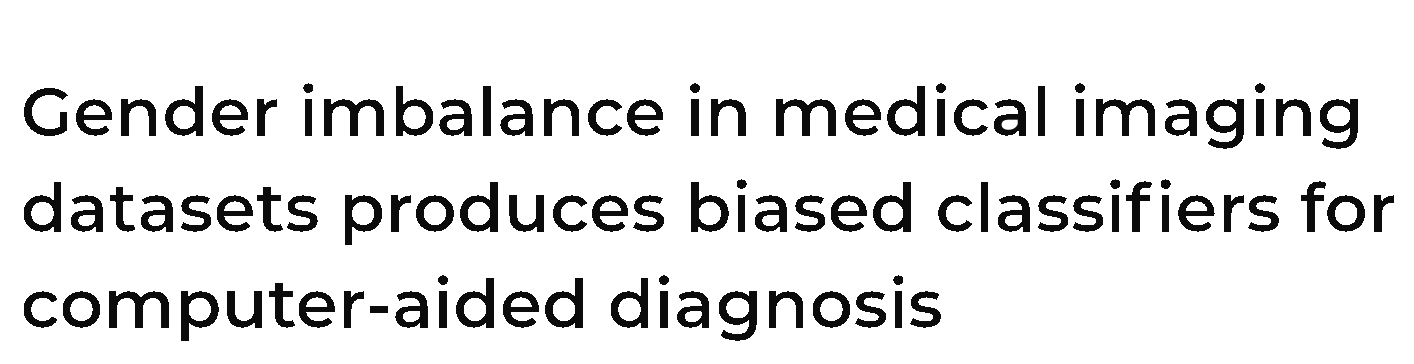
\includegraphics[height=0.2\textheight]{figures/gender_imbalance.png}
 \tiny{www.pnas.org/content/117/23/12592}

 \vspace{1.5cm}

 \textbf{Hiring}

 
\includegraphics[height=0.2\textheight]{figures/hiring.png}
 \tiny{https://interaktiv.br.de/ki-bewerbung/en/}

\end{center}
\end{column}
\begin{column}{0.5\textwidth}
\begin{center}
 \vspace{-0.5cm}

 \textbf{Criminal Justice}

 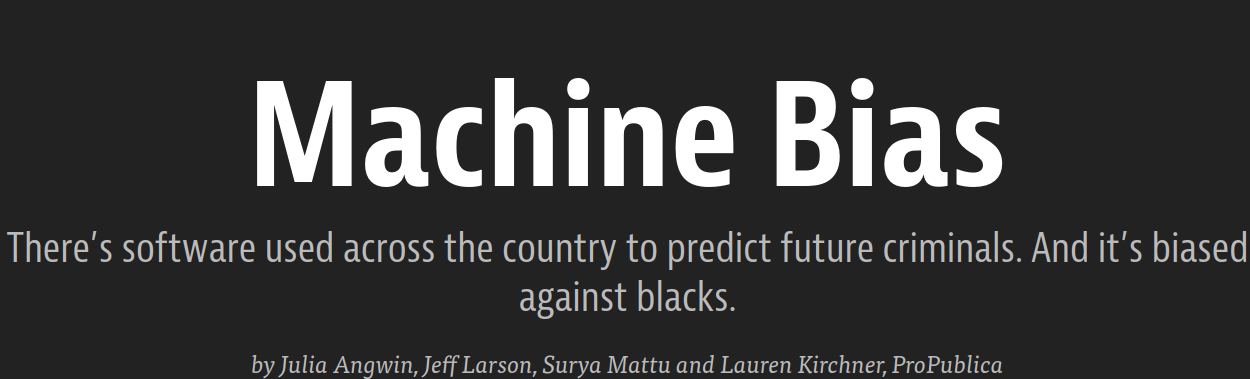
\includegraphics[height=0.2\textheight]{figures/compas.png}
 \tiny{{https://www.propublica.org/article/machine-bias-risk-assessments-in-criminal-sentencing}}

 \vspace{1.5cm}

 \textbf{Search Results}

 
\includegraphics[height=0.2\textheight]{figures/black_girls.png}
 \tiny{https://time.com/5209144/google-search-engine-algorithm-bias-racism/}
\end{center}
\end{column}
\end{columns}
\end{vbframe}


% %% Possibly skip this slide
% \begin{vbframe}{What is Bias?}
% \begin{center}
% \vspace{1.5cm}
% \enquote{Bias as a systematic error or an unexpected tendency to favor one outcome over another}
% (Mehrabi et al., 2019)
% \vspace{1.5cm}
% \enquote{Fairness is the “absence of any prejudice or favoritism towards an individual or a group based on their intrinsic or acquired traits in the context of decision-making}
% (Mehrabi et al., 2019)
% \end{center}
% \end{vbframe}


\begin{vbframe}{Sources of Bias}
\begin{center}
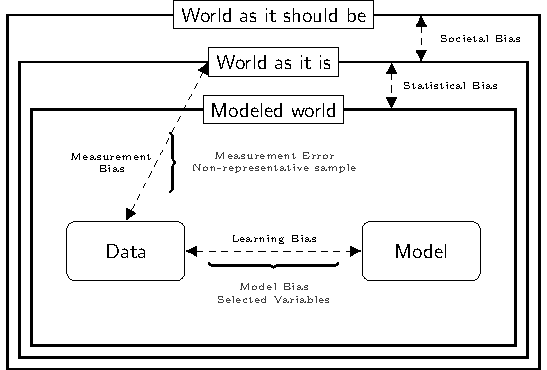
\includegraphics[scale=1]{figures/bias_overview.pdf}
\end{center}
\tiny{Adapted from S. Mitchell et al., Algorithmic fairness: Choices, assumptions, and definitions, 2021}
\end{vbframe}

\begin{vbframe}{Historical Bias}
  \begin{itemize}
  \item Historical data often contains biases, e.g. under-representation of minority groups
  \item Models can pick up existing biases
  \item As a result, biases are perpetuated into the future
  \end{itemize}
  \vspace{1cm}
\begin{center}

\includegraphics[width=0.8\textwidth]{figures/historical_bias.png}

\tiny{Twitter: \@math\_rachel 01.05.2019}
\end{center}
\end{vbframe}

\begin{vbframe}{Representation Bias}
 \vspace{-0.25cm}
  \begin{itemize}
  \item Over- or under-representation of specific sub-population can lead to models that only predict well for majority groups
  \item Models need to be evaluated across a representative sample of the target population
  \item Example: We can only know if a person paid back a loan if we gave out a loan in the first place
  \end{itemize}
\begin{center}
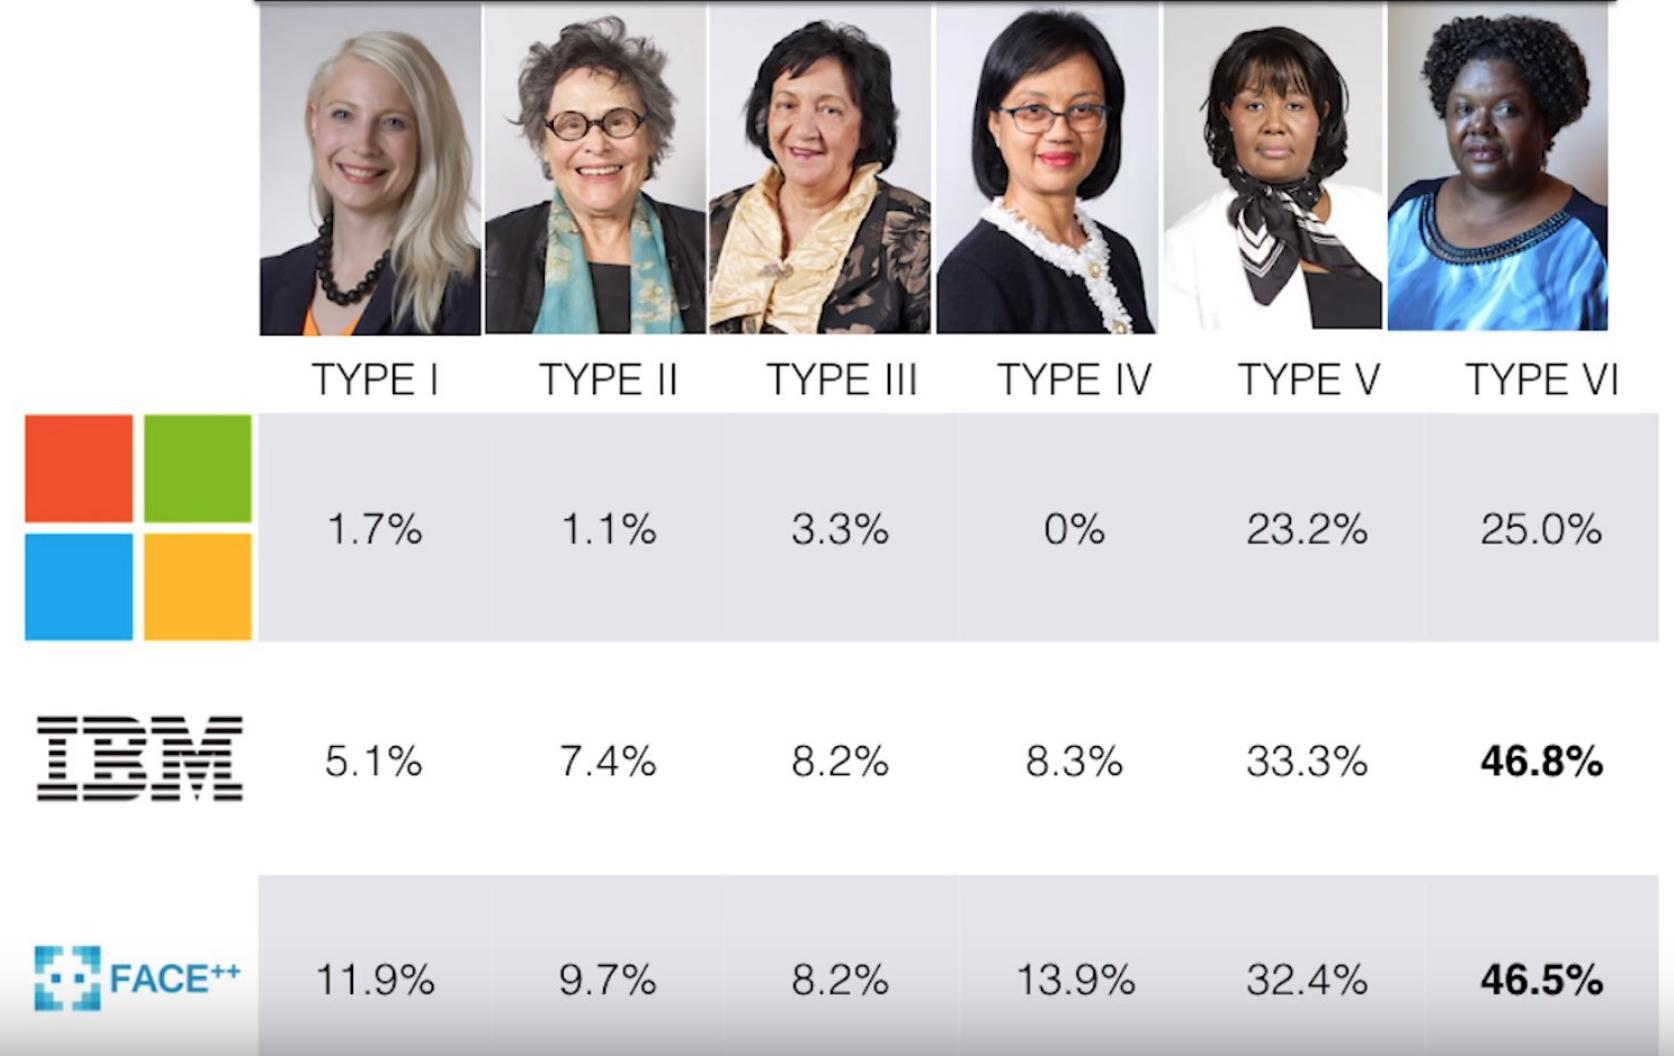
\includegraphics[width=0.6\textwidth]{figures/gendershades.jpeg}

\tiny{gendershades.org}
\end{center}
\end{vbframe}

\begin{vbframe}{Other Sources of Bias}

  \begin{itemize}
  \item \textbf{Measurement Bias} Difference in how a given variable is measured in different sub-populations
    \begin{itemize}
      \begin{footnotesize}
      \item Increased policing in some post codes lead to more prior arrests
      \item Better data quality between different hospitals
      \end{footnotesize}
    \end{itemize}
  \item \textbf{Model Bias} Biases introduced during modelling, e.g. due to under-specified models
      \begin{itemize}
      \begin{footnotesize}
      \item Models make more errors for darker skin tones due to insufficient data
      \item Models pick up spurious correlations in the data
      \end{footnotesize}
      \end{itemize}
  \item \textbf{Feedback Loops} Model decisions shape data collected in the future
      \begin{itemize}
      \begin{footnotesize}
      \item Lead to representation bias if e.g. sub-populations are systematically excluded
      \item People and ML systems 'pick up' miss-representation from search engines. 
      \end{footnotesize}
\end{itemize}
\end{itemize}

\vfill
\tiny{Mehrabi et al., A Survey on Bias and Fairness in Machine Learning, 2020}
\end{vbframe}

\begin{vbframe}{Types of Harms}
  If not accounted for, \textit{biases} can lead to several \textbf{harms}
  \begin{itemize}
  \begin{small}
  \item \textbf{Allocation}: A ressource is allocated unevenly across individuals
  \item \textbf{Quality-of-service}: Systems fail disproportionately for certain groups of individuals.
  \item \textbf{Stereotyping}: Systems re-inforce existing stereotypes
  \item \textbf{Denigration}: Systems are offensive towards individuals
  \item \textbf{Representation}: Under- or overrepresentation of certain groups
  \end{small}
  \end{itemize}

\begin{columns} 
\begin{column}{0.5\textwidth}
\begin{center}
\vfill
 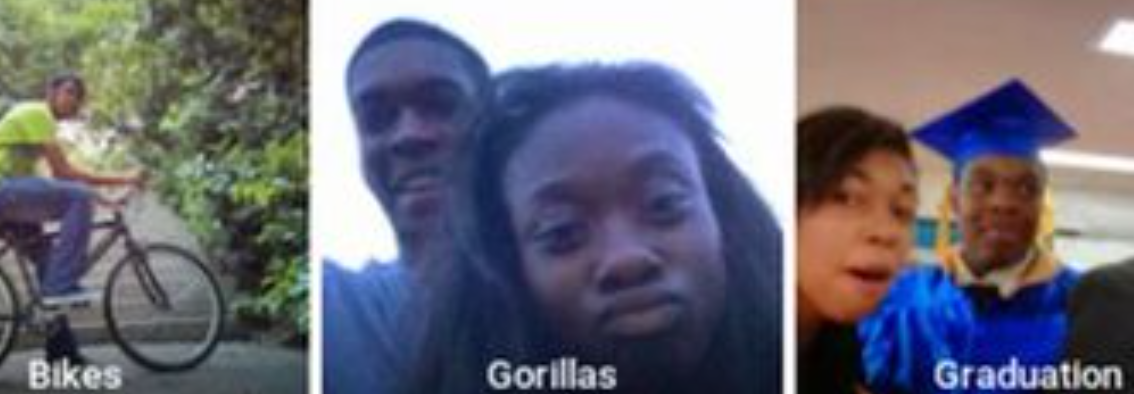
\includegraphics[height=0.25\textheight]{figures/gorilla.png}
 \tiny{Twitter: \@jackyalcine 29.06.2015}
 \vfill
\end{center}
\end{column}
\begin{column}{0.5\textwidth}
\begin{center}
 \vspace{-0.5cm}
 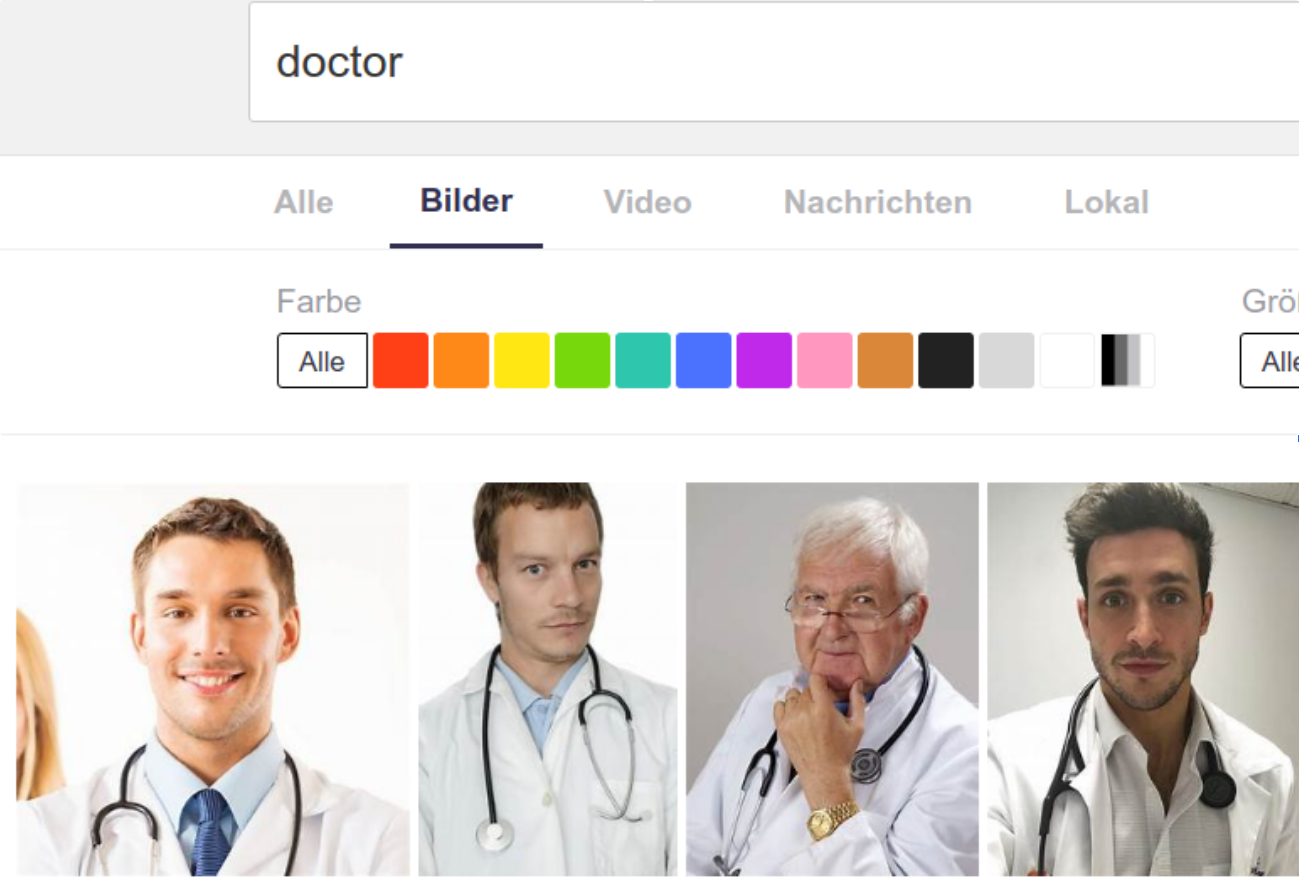
\includegraphics[height=0.3\textheight]{figures/doctor.png}
 \tiny{google.com search for doctor (May, 2021)}
\end{center}
\end{column}
\end{columns}
\vfill
\tiny{H. Weerts, An introduction to algorithmic fairness, 2021}
\end{vbframe}



\begin{vbframe}{Auditing Models for Potential Harms}
  Models Biases in data can have \textbf{ethical}, \textbf{legal} and \textbf{regulatory} consequences \\
  For a more formal treatment, we introduce additional notation:
  \begin{itemize}
    \item \textbf{Protected attribute} Fairness definitions often require a protected \emph{class} or attribute w.r.t which models should be fair.
    We denote this protected attribute $A$ with $\av$. For simplicity, we assume that $\av^{(i)} \in \Aspace = \{0,1\}$ is a binary variable
    \item \textbf{Decision space} In order to make the difference between a model's prediction $\fxh$ and a decision derived from this prediction explicit,
    we denote the decision  with $\dv$. For simplicity, we again assume binary decisions $\dv^{(i)} \in \Dspace = \{0, 1\}$
  \end{itemize}

This notation can be extended to allow for multi-class or regression outcomes as well as more complex protected attributes,
that e.g. allow accounting for non-binary protected classes or \emph{intersectional notions}, e.g. race $\land$ gender.
\end{vbframe}

\begin{vbframe}{Mathematical Notions of Bias - Overview}
\begin{center}
  \vspace{.5cm}
  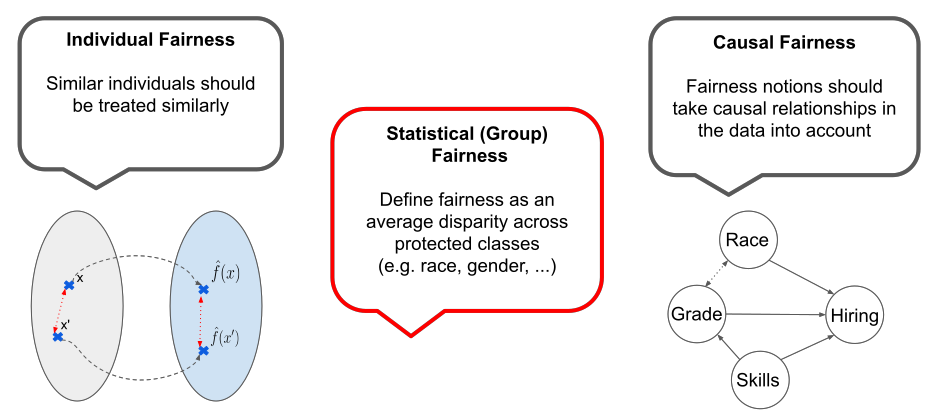
\includegraphics[width=\textwidth]{figures/fairness_definitions.png}
\end{center}
\end{vbframe}

\begin{vbframe}{No fairness through unawareness}
  A naive proposal to reduce harms from ML models is to simply remove the protected attribute.
  \textbf{But:} It's not that simple - models can pick up the information through other variables!
  \vspace{-.4cm}
  \begin{columns} 
    \begin{column}{0.5\textwidth}
    \begin{center}
    \textbf{Direct Discrimination}
    \vspace{.2cm}
    \begin{tikzpicture}
      % x node set with absolute coordinates
      \node[state] (a) at (0,0) {$Race$};
      \node[state] (x1) [right =of a] {$ZIP$};
      \node[state] (x2) [right =of x1] {$Income$};
      \node[state] (y) [below =of x1] {$Credit$};
      % Directed edge
      \draw [->, red] (a) -- (y);
      \draw [->] (x1) -- (y);
      \draw [->] (x2) -- (y);
    \end{tikzpicture}
    \end{center}
    \vfill
    $\rightarrow$ The model directly uses race as a feature.
    \end{column}
    \begin{column}{0.5\textwidth}
      \begin{center}
        \textbf{Indirect Discrimination}
        \vspace{.2cm}
        \begin{tikzpicture}
          % x node set with absolute coordinates
          \node[state] (a) at (0,0) {$Race$};
          \node[state] (x1) [right =of a] {$ZIP$};
          \node[state] (x2) [right =of x1] {$Income$};
          \node[state] (y) [below =of x1] {$Credit$};
          % Directed edge
          \draw [->, red] (a) -- (x1);
          \draw [->] (x1) -- (y);
          \draw [->] (x2) -- (y);
        \end{tikzpicture}
        \end{center}
    \vfill
    $\rightarrow$ The model picks up information about the race through the proxy-variable ZIP-code.
    \end{column}
    \end{columns}
  \vfill
\end{vbframe}

\begin{vbframe}{Group fairness definitions}
  Several fairness definitions based on differences between protected groups have been proposed.
  \begin{itemize}
    \item \textbf{Statistical Parity}: The chance to get the favourable outcome is equal across two groups. This is also 
          called \textit{demographic parity}.
          \[
          P(\hat{Y} = 1 | A = 0) = P(\hat{Y} = 1 | A = 1)   
          \]
    \item \textbf{Equalized Opportunity}: The chance to \emph{correctly} be assigned the favourable outcome is independent of 
          the protected attribute. 
          \[
            P(\hat{Y} = 1 | A = 0, Y = 1) = P(\hat{Y} = 1 | A = 1, Y = 1)   
          \]

    \item \textbf{Accuracy Parity}: The accuracy is equal in both groups.
    
    \[ \begin{aligned}
    & P(\hat{Y} = 1 | A = 0, Y = 1) + P(\hat{Y} = 0 | A = 0, Y = 0) = \\
    & P(\hat{Y} = 1 | A = 1, Y = 1) + P(\hat{Y} = 0 | A = 1, Y = 0)
    \end{aligned} \]
  \end{itemize}
\end{vbframe}

\begin{vbframe}{Perspective: Based on predicted outcome}
    \textbf{}
    \begin{itemize}
      \item Statistical parity requires equality in the predicted outcome.\\
      E.g. hire candidates \textbf{independent} of qualification.
      \item If the underlying qualifications are not distributed equally across groups, we need to sacrifice \emph{utility} to achieve statistical parity.
    \end{itemize}
    \begin{center}
      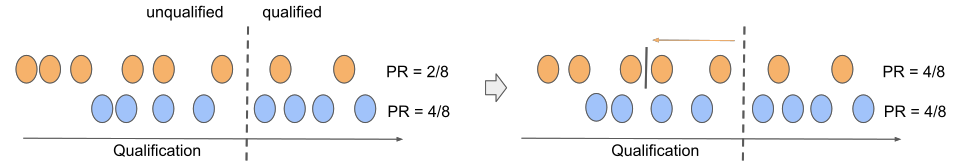
\includegraphics[]{figures/statistical_parity}
    \end{center}
    $\rightarrow$ Enforcing equal positive rates might require hiring unqualified candidates.\\
    \textbf{Danger:} If the bias comes from the real world (e.g. societal bias), enforcing statistical parity can also lead to adverse effects in the long term.
\end{vbframe}

\begin{vbframe}{Perspective: Based on true \& predicted outcome}
  \textbf{}
  \begin{itemize}
    \item Other fairness notions require equality of some error notions, e.g. false positive rates.\\
    E.g. hire \emph{qualified} candidates at equal rates across groups.
    \item Error based notions are often more intuitive and easy to communicate.
    \item Can help to idenitify representation or model bias
    \item Error based notions do not account for systemic injustices in the world -- if e.g. labels are biased, we can still be \emph{fair} according to error-based notions. 
  \end{itemize}
\end{vbframe}

\begin{vbframe}{Reminder: Confusion Matrix}
  The confusion matrix is a $2 \times 2$ contingency table of predictions $\hat{y}$ and true labels $y$.
  Several evaluation metrics can be derived from a confusion matrix:
  \vfill
  \begin{center}
  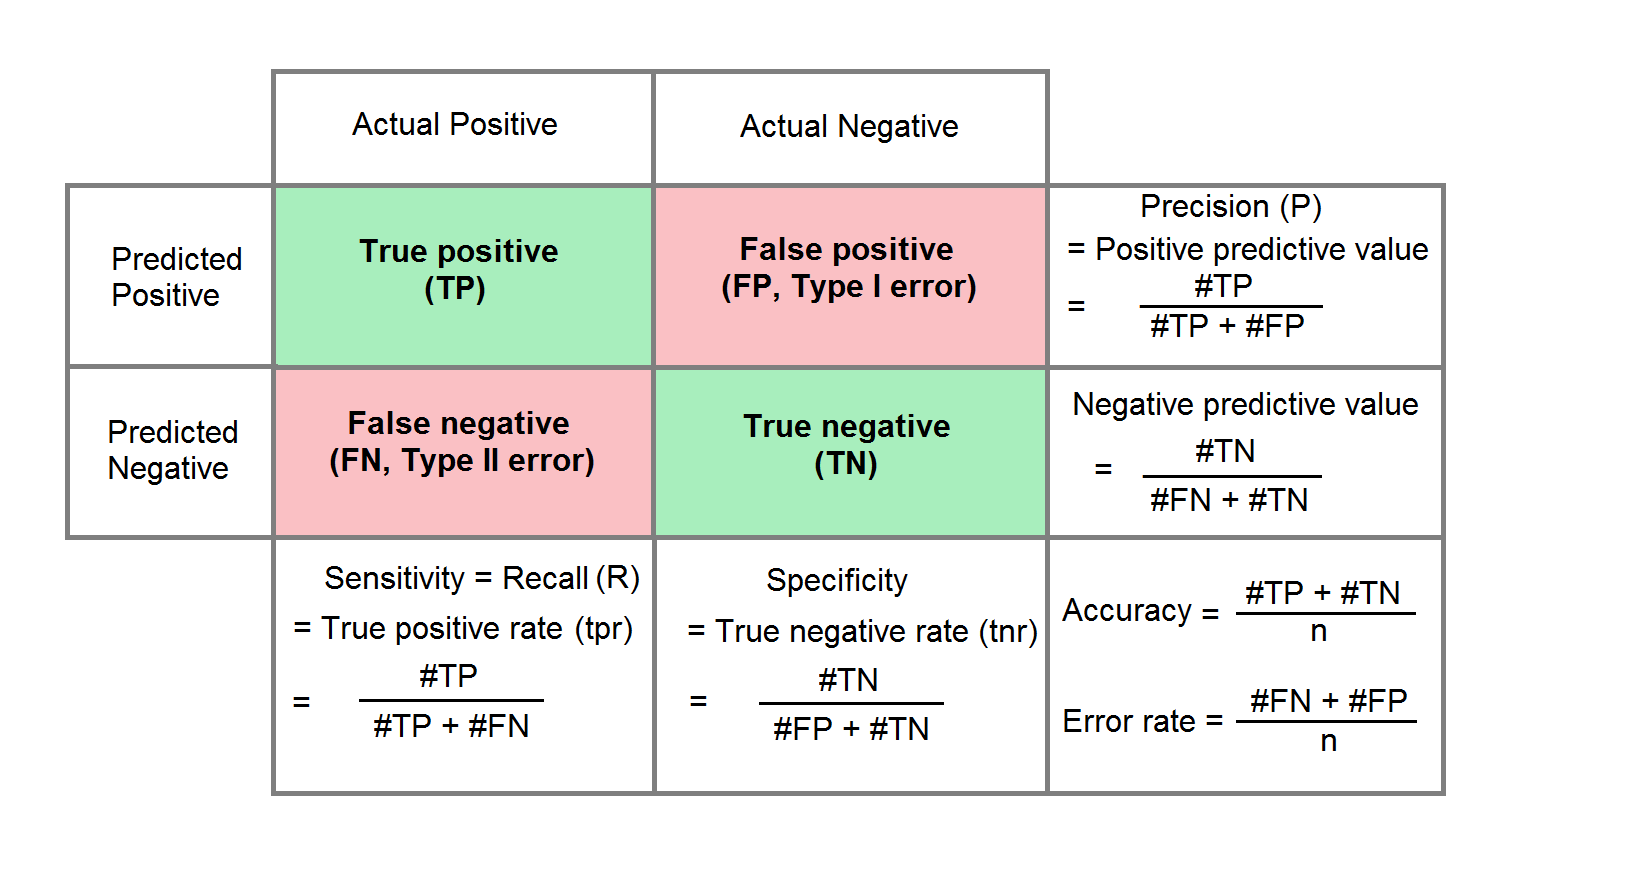
\includegraphics[width=0.8\textwidth]{figures/roc-confusion_matrix.png}
  \end{center}
  $\rightarrow$ Many fairness metrics can be expressed as entries of the confusion matrix
\end{vbframe}
   
\begin{vbframe}{Fairness Tensor}
  We can represent labels \& predictions as a \emph{fairness tensor} (Kim et al., 2020).
  Fairness tensors are 3-dimensional, stacked confusion matrices:

  \[
  Z = \left[
    \begin{bmatrix}
    TP_1  & FP_1 \\
    FN_1  & TN_1
    \end{bmatrix} ^{A=1}
    ,
    \begin{bmatrix}
      TP_0  & FP_0 \\
      FN_0  & TN_0
    \end{bmatrix} ^{A=0} 
    \right]
  \]
  \vspace{.2cm}
  For $z = (TP_1,FN_1,FP_1,TN_1,TP_0,FN_0,FP_0,TN_0)^T / N$, we can express a large variety of fairness metrics as 
  linear $\phi(x) = A \cdot z$ or quadratic functions $\phi(x) = z^T \cdot B \cdot z$ by choosing an appropriate matrix $A$ or $B$. \\
  \vspace{.2cm}
  \textbf{Example:} \\ We choose $A = (N_1, 0, N_1, 0, N_0, 0, N_0, 0) / N$, where $N_{a}$ is the sum of entries in the confusion matrix for protected grou $a$.
  We can now express \textbf{statistical parity} as $A \cdot z = 0$.
\end{vbframe}
\begin{vbframe}{Incompatibility of Fairness Metrics}

  Some fairness metrics can not be jointly satisfied, except for trivial settings.
  As a result, we can not build a universal fairness metric that satisfies all fairness requirements.
  This has been shown for several combinations of fairness metrics, e.g. equal true positive, false positive and false negative rates.\\
  \vspace{.2cm}
  We can formally show this using the fairness tensor $z$ and matrices $A_{TPR}, A_{FPR}, A_{FNR}$ encoding the fairness metrics.
  Showing that fairness metrics are compatible now requires showing that the system of equations 
  \[ \begin{bmatrix} A_{TPR} \\ A_{FPR} \\ A_{FNR} \end{bmatrix} \cdot z  = \begin{bmatrix} 0 \\ 0 \\ 0 \end{bmatrix} \]
  has a solution. If no solution $z$ exists, the metrics are incompatible.

\end{vbframe}

\begin{vbframe}{Fairness Metrics - Closing Thoughts}
  \begin{itemize}
    \item Statistical group fairnes metrics require translating ethical considerations of what is \emph{fair} into mathematical formulas.
    \item To draw meaningful conclusions, we need to evaluate fairness metrics on a \textbf{representative} data set. 
    \item Fairness metrics reduce a wide variety of important considerations into a single number -- they are not designed to guarantee that a system is fair.
    \item Incompatibility between fairness metrics implies that we might need trade-offs between fairness metrics.
  \end{itemize}
\end{vbframe}

\begin{vbframe}{Preventing \& Mitigating Harms - Documentation}
    Harm from machine learning models can often be prevented by improving documentation of existing datasets \& models.
    To provide an example, usage of datasets or models outside of their intended use can often lead to harm, even if the models are carefully validated.
    \begin{itemize}
      \item \textbf{Dataset documentation} Includes information on the dataset, sampling mechanisms and intended use.
      Can inform model developers on possible representation biases or other problems with the data. \\
      \textbf{Example:} Datasheets for datasets
      \item \textbf{Model documentation} Includes information about the model, used data and hyperparameters. 
      Can inform users on the relevant performance metrics, intended use of a given model. \\
      \textbf{Example:} Modelcards for ML models
      \item \textbf{Fairness reports} Include information about performed fairness audits.
    \end{itemize}
\end{vbframe}

\begin{vbframe}{Preventing \& Mitigating Harms - Bias Mitigation}
  Several \emph{bias mitigation techniques} have been proposed:
  \begin{itemize}
    \item \textbf{Pre-processing}: Transform data to make subsequently trained models fairer.
    \item \textbf{In-processing}: Learn a model that directly incorporates fairness constraints.
    \item \textbf{Post-processing}: Adapt model predictions to satisfy fairness constraints.
  \end{itemize}
  \textbf{Example:}\\
  Re-weighing (Kamiran, 2012) proposes to use sample weights that are inverse to the frequency of labels and predictions in the data.
\end{vbframe}

\begin{vbframe}{Preventing \& Mitigating Harms - Recourse}
  Fair treatment of individuals subject to a decision making systems decisions can often not only be achieved solely through algorithmic means
  but requires recourse, accountability \& interpretability.
  \begin{itemize}
    \item \textbf{Accountability}: Automated systems will make errors - developers need to ensure that humans responsible for addressing such errors exist and have the means to address such errors.
    \item \textbf{Interpretability}: Interpretability techniques can help to identify possible problems in the data or the model, e.g. spurious correlations picked up by the model.
    \item \textbf{Recourse}: Individuals subject to automated decisions should have access to an explanation on how the decision was made and what steps can be taken to address unfavourable predictions.
  \end{itemize} 
\end{vbframe}


\begin{vbframe}{Further considerations}
  \begin{itemize}
    \item \textbf{Intersectionality}: Fairness considerations should often hold across intersectional groups, e.g. $race \land gender$.
    \item \textbf{Intervention design}: Instead of ensuring a given intervention is fair, it can often be helpful to consider the intervention we wish to deploy. \\
    \textbf{Example:} Instead of penalizing defendants for not showing up to court, provide them with means of transportation.
    \item \textbf{Stakeholder participation:} Developing ML models should take the perspective of all stakeholders such as the individuals affected by the intervention and advocacy groups.
    \item \textbf{Long-term perspective:} Existing metrics only consider the short-term and do not take its long-term impact into account. This might lead to adverse effects in the long-term.
  \end{itemize}
\end{vbframe}

\begin{vbframe}{Resources}
\begin{itemize}
\item Fairness and Machine Learning - Limitations and Opportunities, Barocas et al., 2019
\item Algorithmic Fairness: Choices, Assumptions, and Definitions, Mitchell et al., 2021
\item A Survey on Bias and Fairness in Machine Learning, Mehrabi et al., 2020
\item An Introduction to Algorithmic Fairness, H.J.P Weerts, 2021
\item FACT: A Diagnostic for Group Fairness Trade-offs, Kim et al., 2020
\item Data preprocessing techniques for classification without discrimination, Kamiran et al., 2012
\item Fairness Through Awareness, Dwork et al., 2012
\end{itemize}
\end{vbframe}

\begin{vbframe}{Software}
  \begin{itemize}
  \item \texttt{fairlearn} (Python)
  \item \texttt{aif360} (Python)
  \item \texttt{fairmodels} (R)
  \item \texttt{mlr3fairness} (R)
  \end{itemize}
  \end{vbframe}

\endlecture
\end{document}